
\section{Introduction}
\label{sec:Introduction}
why network virtualization is significant.

network virtualization has gained significant attention in recent years as an effective means to share substrate network (SN) infrastructure among several virtual network (VN) service providers so as to improve the utilization of the substrate resources \cite{armbrust2009above,yu2008rethinking}. In the network virtualization environment, provisioning a VN is a promising way to support distributed applications and services which require the coordination of multiple geographically distributed facilities (e.g. storage arrays or computer clusters). With the maturity of the optical network technology and their high-bandwidth and low-latency characteristics, we will be able to deploy a federated computing and networking system (FCNS) \cite{zhang2013effective,papagianni2013optimal}, which interconnects a large number of facility nodes with optical network managed or controlled integratedly, to enable such large scale distributed applications.

Network virtualization is a promising technology to reduce the operating costs and management complexity of networks, and it is receiving an increasing amount of research interest\cite{chowdhury2009network}. Survivability is bound to become a more prominent issue as infrastructure providers move toward virtualizing their networks over cheaper commodity hardware\cite{bhatia2008trellis}. we are concerned with critical virtual nodes and embedding them as an entire infrastructure with survivability guarantees. Fault tolerance is provided in data centers \cite{guo2009bcube} through excessive redundant nodes and links organized in a special way. These works provide Survivability but do not customize survivability guarantees to embedded VInfs. However, such slice is not used as a back-up, but as a monitoring tool, and as a way to debug
the network in the case of failure.\cite{wang2008virtual} considered the use
of virtualized router as a management primitive that can be used to migrate routers for maximal reliability.

what is VN

In network virtualization, the primary entity is the Virtual Network (VN). A VN is a combination of active and passive network elements (network nodes and network links) on top of a Substrate Network (SN). Virtual nodes are interconnected through virtual links, forming a virtual topology. By virtualizing both node and link resources of a SN, multiple virtual network topologies with widely varying characteristics can be created and co-hosted on the same physical hardware.
Each VN request consists of a collection of virtual (task) nodes connected together by a set of virtual links to form a virtual topology; it also has certain resource requirement, such as computing resources for the nodes and bandwidth resources for the links. Such VN request could be represented by a task graph. To establish the VN, one needs to embed task nodes onto facility nodes, and virtual edges onto one or more substrate paths\cite{yu2008rethinking} , as well as allocating sufficient substrate resources which should not violate the computing/ bandwidth capacity limits of facility node/substrate link.



why node failure happern

With infrastructure rapidly becoming virtualized, shared and dynamically changing, it is essential to have strong reliability support from the physical infrastructure, since a single physical server or link failure affects several shared virtualized entities. Providing survivability is often linked with over-provisioning both computational and network capacities, and employing load balancing for additional robustness. Such highly survivable systems are good for applications where large discontinuity may be tolerable, e.g. restart of network flows while rerouting over link or node failures, or partial job restarts at node failures. A higher level of fault tolerance is required at applications where some failures have a substantial impact on the current state of the system. For instance, virtual networks with servers which perform admission control, scheduling, load balancing, bandwidth broking, AAA or other NOC operations that maintain snapshots of the network state, cannot tolerate total failures. In master slave/ worker architectures, e.g. MapReduce, failures at the master nodes waste resources at the slaves/workers, we do not talk about the capacity requirement and geographical location requirement of virtual node, and the bandwidth capacity requirement of virtual link in this paper.

what situation happen

In the multi-tenant network virtualization environment, one challenging problem raised is how to efficiently embed VN requests with various constraints. This is of utmost importance for increasing the utilization of SN resources and infrastructure providers’ revenue \cite{koponen2014network}. Survivable virtual network embedding deals with failures in the substrate and virtual network. The challenges to be considered are link and node failures, which have to be backed up before the failure or recovered after failure. Failures can occur at different layers in the network. For example at the physical layer, a fiber cut
may cause a physical dis-connectivity. In\cite{markopoulou2004characterization}, it is shown that 20 \% of all failures in an IP backbone are resulting from
maintenance activities. About 53 \% of the unplanned link failures are due to router-related \cite{markopoulou2004characterization}. In a network, single
and also multiple failures can occur. The single failure case happens more often than multiple simultaneous failures. The study \cite{markopoulou2004characterization} states that about 70 \% of the unplanned link failures are single link failures. A study \cite{gill2011understanding} about network-related failures in data centers found out that link failures happen about ten times more than node failures per day. Usually node failures are due to maintenance \cite{gill2011understanding}.


why survivable eVN is paramount

However, with network virtualization gaining momentum, the survivability challenges in VNE should also be well investigated. In a large networked computing system, hardware and software failures of facility nodes and communication resources (e.g., links and switching nodes) are norm instead of exception, such as power outages caused by virus attack, disk failures, misconfiguration or fiber cut \cite{xu2012survivable,rahman2010survivable,rahman2013svne,guo2011shared,chen2010resilient}. Such failures will force the virtual node (links) assigned to it to be migrated/re-embeded to another facility node at a geographically different location (link disjoint substrate path). This means that, in order to survive from the disruptions due to such failures, one must reserve redundant facility nodes and bandwidth on fiber links such that after any failure when virtual network request had been embedded in substrate network, there are adequate remaining computing and networking resources to migrate/remap the eVN request. In most case, failure occur when VN had been embedded into SN. Accordingly, the problem of minimizing the resources, including computing and communication resources, reserved for VN request to tolerate substrate failures, (hereafter called Survivable eVN problem, SeVN) is both critical and challenging. Actually, SeVN problem is quite different with the protection approach
in IP over WDM network by investigating facility node failure caused virtual node failure problem and employing node migration induced VN remapping as an unique recovery strategy.


why happen Survivable embeded Virtual Network Request

The software-defined NFV architecture further offers agile traffic steering and joint optimization of network functions and resources.
%When a survivable request of virtual network is coming, survivable virtual network requests are associated with node's service functions.
In any real virtual networks, any nodes of virtual network  are deployed with a service function and the corresponding physical node could run some various service functions. After virtual network VN is embedded into substrate network, a running node of physical network could fail multiple virtual network so that we should obtain survivable eVN to be embedded into substrate network so that recovery from the failure even though one or multiple nodes of virtual network failed because these virtual node corresponding substrate node fail. The augmented nodes of survivable embedded virtual network are embedded into substrate network ultimately, the augmented nodes have specific service functions similarly as shown in Fig.\ref{fig:VNmapSN}.

\begin{figure}
  \centering
  % Requires \usepackage{graphicx}
  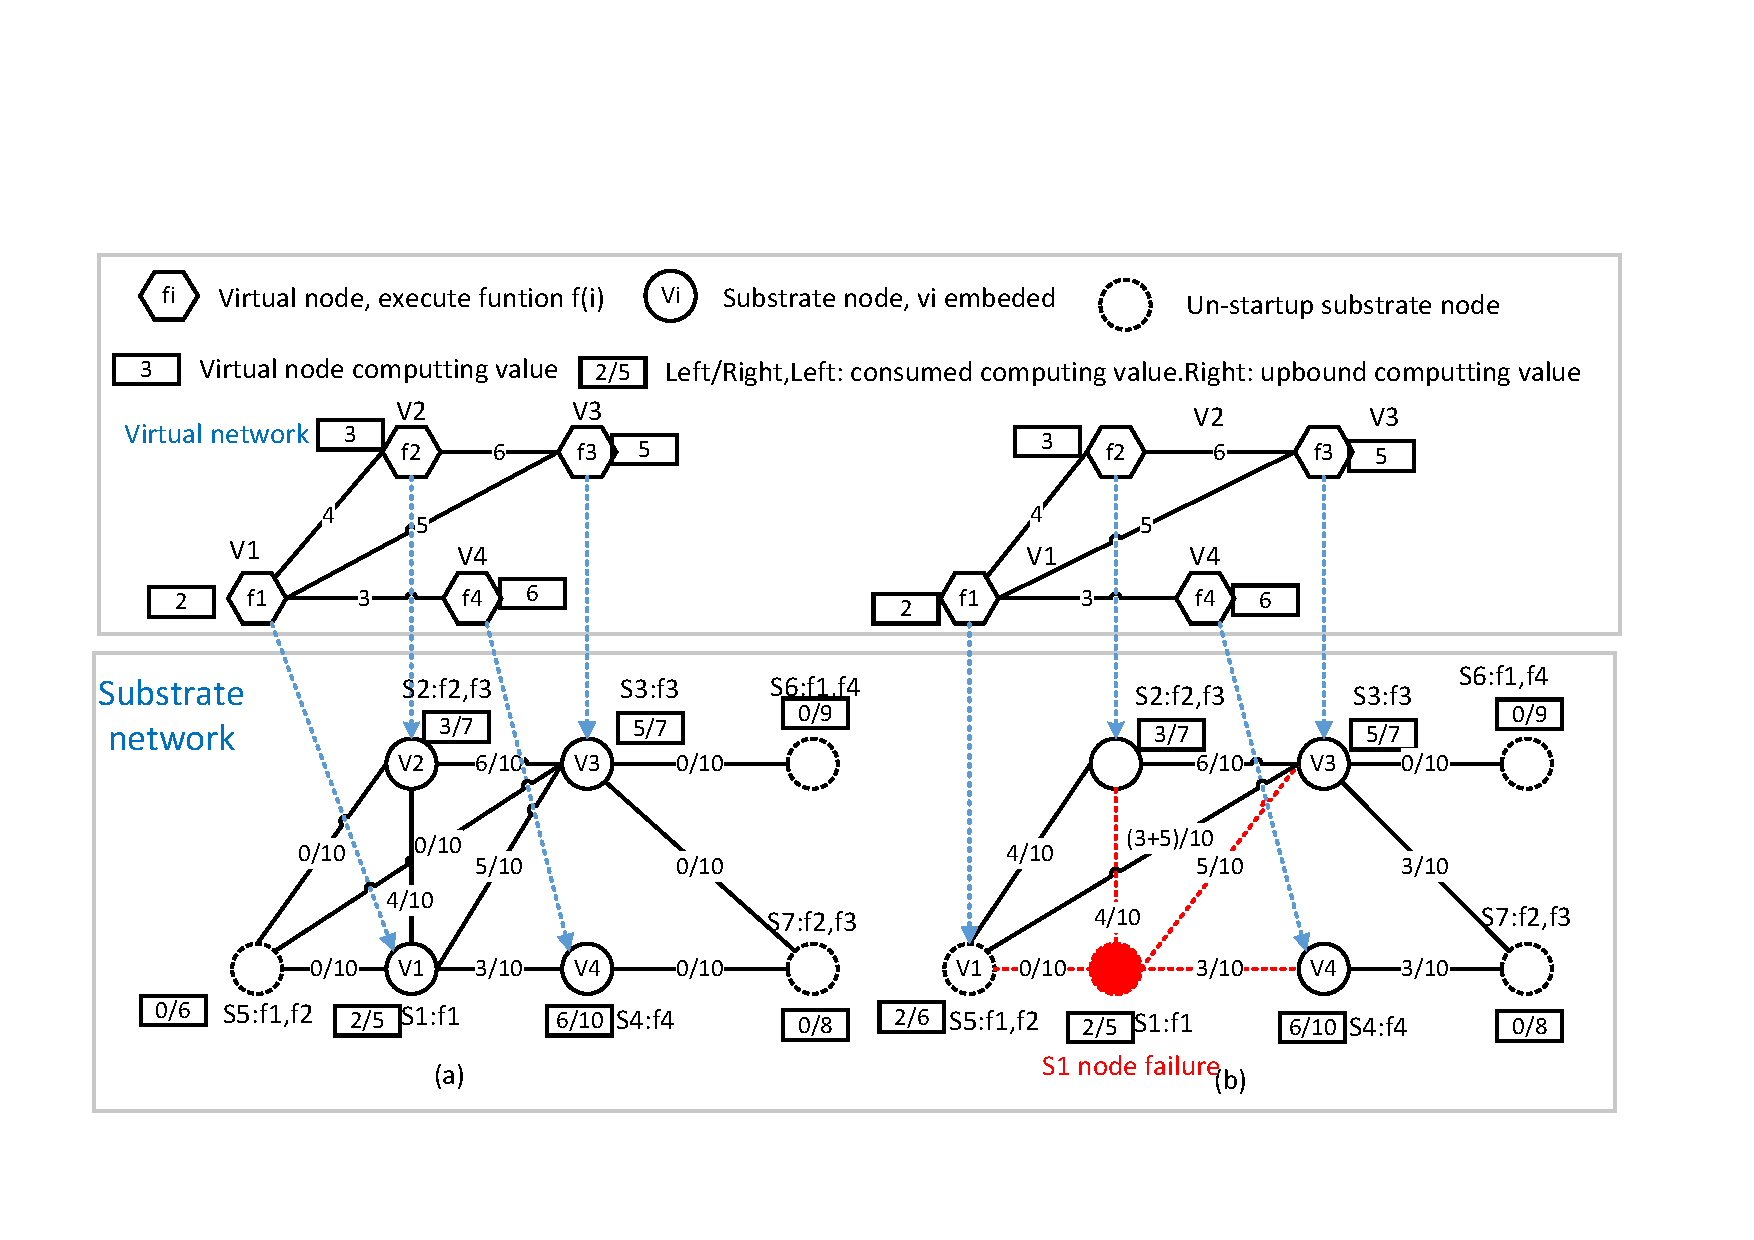
\includegraphics[width=3in]{Fig/VNmapSN}\\
  \caption{function virtual network (VN) embedding and one node failure}\label{fig:VNmapSN}
\end{figure}

proactive or reactive type

There are two main survivability methods: protection and restoration \cite{ramamurthy2003survivable}. Failure protection is done in a proactive way to reserve the backup resources before any failure happens. Reactive mechanisms, which are called restoration mechanisms, react after the failure occurs and start the backup restoring mechanism. However, some data loss is possible in the reactive case. There exist two kinds of backups for the protection scheme: dedicated backup or shared backup. In shared backup, the resources for the backup may be shared with other backups. In the dedicated case the backup resources are not shared for other backups.


To survive a substrate link failure, pre-computed alternative paths inVN are used in general and the bandwidths are allocated before or after a failure. For instance, the reactive detour solution is employed after a substrate link failure in \cite{rahman2010survivable}, while authors in \cite{rahman2013svne,guo2011shared} propose a proactive backup approach (considering the backup resources sharing) to avoid service disruption in reactive restoration approach and improve the substrate resource utilization.


FD  FI

In terms of SeVNE capable of recovering/re-embedding the task nodes after a facility node failure, there are two basic approaches: Failure Dependent Protection (FDP \cite{yu2010survivable} and Failure Independent Protection (FIP) \cite{yeow2011designing}, and the differences between them are as follows. In FIP, a host (facility) node is assigned and dedicated to backup all working host (facility) nodes. That is, no matter which working host node fails, the affected task node will be migrated to the only one backup host node. On the other hand, with FDP, each working host node can have a different backup host node under different failure scenarios. In fact, after a failure, even an unaffected task node may be migrated from a working host node to its corresponding backup host node, as a result of re-embedding the entire task graph. In other words, FDP could provide more flexibility in survivable VN designing by allowing task nodes migrating freely after failure, so FIP could be considered as a special case of FDP and FDP is expected to use fewer resources at the cost of more task nodes migrations after a failure.


Guarantying integration of topological structure of virtual network request is more important than node migration cost when facility node failure.


serive type

Through synchronization\cite{bressoud1996hypervisor,cully2008remus} and migration techniques\cite{clark2005live,wang2008virtual} on virtual machines and routers, we suppose that every virtual network have specific service functions, in addition that fault tolerant can be introduced at the virtualization layer\cite{yeow2011designing}. \cite{qu2016delay}

node cost larger than edge cost

As nodes often represent expensive components (servers) and edges represent less expensive interconnections (links) \cite{armbrust2009above,yu2010survivable}, most attention has been devoted to node faults, i.e., the removal of nodes (and their incident edges), rather than edge faults where only edges are removed.

The node failure type we focus in this paper is independent node failures. multiple independent or dependent failure nodes problem could be discussed in the future. 


%
%\begin{table}
%\centering
%\begin{tabular}{cc}
%\hline
%Term & Description \\
%$G(V,E,S)$ & $G(V,E,S)$ denotes the Virtual Network, consisting of nodes V, links E and service functions\\
%$B(V,S)$ & $B(V,S)$ denotes the Backup nodes set, consisting of nodes V and service functions S which is corresponding to every nodes \\
%\hline
%\end{tabular}
%\caption{terminology used throughout this paper}\label{tab:term}
%\end{table}

The organization of this paper is as follow. In the next section, we briefly describe the background, notations and define survivability in Sec.\ref{sec:ProblemFormulation}. Finally, we evaluate and validate the ideas through simulation in Sec.\ref{sec:Evaluation}. 